%-------------------------------------------------------------------------------
% HAP
%-------------------------------------------------------------------------------
\documentclass{ipol}
\ipolSetTitle{HAP: Hierarchical Affinity Propagation}
\ipolSetAuthors{Nelle Varoquaux, Raphael Grompone Von Gioi}
\ipolSetYear{2012}
\ipolSetMonth{3}
\ipolSetDay{1}
\ipolSetID{gjmr-lsd}

\usepackage{hyperref,verbatim,graphicx,amsmath,amssymb,amssymb,dsfont}
\usepackage[ruled,linesnumbered]{algorithm2e}
\newtheorem{theorem}{Theorem}


\DeclareMathOperator{\argmax}{argmax}
\bibliographystyle{acm}

\begin{document}

%-------------------------------------------------------------------------------
\begin{abstract}

Clustering data by finding representative points is an important task of data
analysis. \cite{frey07affinitypropagation} introduces a novel algorithm based
on passing messages to find such points, called "exemplars". \cite{hap}
extended this algorithm to find hierarchical layers of exemplars. We present
this method, called Hierarchical Affinity Propagation (HAP).

\end{abstract}

%-------------------------------------------------------------------------------
\begin{ipolCode}
\end{ipolCode}

%-------------------------------------------------------------------------------
\begin{ipolSupp}
\end{ipolSupp}

%-------------------------------------------------------------------------------
\section{Introduction}
%-------------------------------------------------------------------------------

% XXX rephrase
Findings a small number of points that represents well a dataset is a critical
step in pattern recognition. Exemplar-based clustering performs not only a
clustering step, ie partitionning a set of datapoints that are similar in some
sense, but also identifies for each cluster a point which represents the most
that clusters. Those points are called "exemplars". \\
Clustering can be done by randomly choosing a number of points from
the dataset, and iteratively refining clusters. Such methods, sensitive to the
initialization, often fall in local minima, and have to be reran several
times.\\
Affinity propagation (AP) takes a novel approach, and considers all datapoints
as potential exemplars. By passing messages reflecting the affinity between
datapoints, clusters emerge gradually from the dataset. \\

\section{Affinity Propagation}
Let $N$ be the number of datapoints.

Affinity propagation takes in input two elements: \textbf{similarities} and
\textbf{preferences}. The similarity $s_{ij}$ defines how well $j$ is suited
to be $i$'s exemplar, ie how much $i$ and $j$ are similar. Affinity
propagation does not require similarities to be symmetric. Intuitively,
similarities $s_{ij}$ can be set to the negative euclidean distance between
two points. \\

The preference $p_i$ sets how well $i$ is likely to be chosen as exemplar. Low
preferences will yield a smaller number of exemplars, while high preferences
will yield a large number of exemplars. Thought in some application, setting
different preferences to point may be justified, there is often little reason
to favor a priori one point other another. Hence, preferences can be set as
the median for an average number of clusters, or to the minimum of the
similarities, for a small number of clusters. \\

Let $e_j$ be a set of hidden variable, where $e_j = 1$ indicates that point
$j$ has been chosen as an exemplar. Let $h_{ij}$ be a set of hidden variable
that chose that point $i$ has chosen point $j$ as it's exemplar. We can now
set some constraints:
\begin{itemize}
\item One point can choose only one exemplar:
\begin{equation*}
\sum_{j} h_{ij} = 1
\end{equation*}
\item If a point is an exemplar, than it is necessarily it's own exemplar
\begin{equation*}
e_{j} = 1 \Rightarrow h_{jj} = 1
\end{equation*}
\end{itemize}

We can express the optimization problem as:
\begin{equation*}
\renewcommand{\arraystretch}{2}
\begin{array}{ccll}
\text{maximise} & & \sum_{i, j} s_{ij} h_{ij} + \sum_{j} p_j e_j & \\
\text{subject to} &  & \sum_{j} h_{ij} = 1, & i = 1, \dots, n \\
		  &  & e_{j} = h_{jj}, & j = 1, \dots, n\\
\end{array}
\end{equation*}


The second term of the objective function is a penalty term on the number of clusters, preventing the
trivial solution of each point picking itself as exemplars. The higher the
preference is, the more important the penalty on a point will be, the lower
the probability of choosing this point as an examplar will be. This problem is
NP hard. Hence, we will use an iterative and approximate algorithm inspired
from the max sum algorithm to find exemplars. \\

Two notions are derived from the similarities and preferences:
\textbf{responsibilities} and \textbf{availabilities}. These two types of
messages are computed iteratively until convergence.
\\
The responsibility $r_{ik}$ of data point $i$ to
candidate exemplar $j$ corresponds to how well $k$ is suited to be an exemplar
for $i$, compared to all the other exemplar candidates. The higher the
similarity between points $i$ and points $j$, the higher should the
responsibility be.
\begin{equation*}
r_{ij} = s_{ij} - \max_{k \neq j} (a_{ik} + s_{ik})
\end{equation*}
\\
The availability $a_{ik}$ of candidate exemplar $k$ to point $i$ shows how
appropriate it is for $i$ to choose point $k$ as an exemplar; it takes in account
all the other points $j$ that would take $k$ as an exemplar. The
self-availability $a_{kk}$ reflects the probability that point $k$ is an
exemplar based on the positive responsibility send from all points to $k$.

\begin{equation*}
a_{ij} = \begin{cases}
	    p_j + \sum_{k \neq j} \max(0, r_{kj}) &  i = j \\
	    \min ( 0, p_j + r_{jj} + \sum_{k \notin \{i, j\} } \max (0, r_{ij}))
	    & i \neq j\\
	 \end{cases}
\end{equation*}

$(a_{ij} + s_{ij})$ defines the certainty of $i$ choosing $j$ as exemplar.
Hence:
\begin{equation*}
e_i = \arg \max_j a_{ij} + s_{ij}
\end{equation*}

\begin{algorithm}[h]
  \SetLine
  initialization\;
  \For{iteration}{
    Compute availabilities $a_{ij} = \begin{cases}
	    p_j + \sum_{k \neq j} \max(0, r_{kj}) &  i = j \\
	    \min ( 0, p_j + r_{jj} + \sum_{k \notin \{i, j\} } \max (0, r_{ij}))
	    & i \neq j\\
	 \end{cases}$\;
    Compute responsibilities $r_{ij} = s_{ij} - \max_{k \neq j} (a_{ik} + s_{ik})$\;
  }
  Compute exemplars $e_i = \arg \max_{j} a_{ij} + s_{ij}$ \;
  \caption{Affinity Propagation}
\end{algorithm}

\begin{figure}
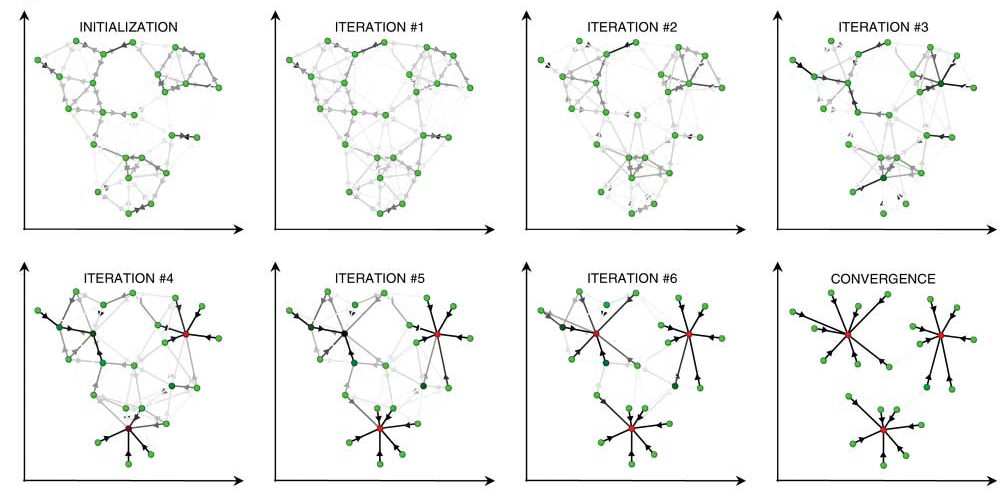
\includegraphics[width=500px]{./images/AP_frey.png}
\caption{Message passing between evolution over iteration.}
\end{figure}

\section{Hierarchical Affinity Propagation}

The affinity propagation algorithm can be generalized in a hierarchical
clustering algorithm. Let $L$ be the number of layers. All exemplars at layer
$l$ should also be exemplars at level $l -1$. Hence, number of exemplars
should decrease when going up the layers, and one exemplar at level $l$ can
either stay an exemplar at level $l + 1$ or chose another exemplar to be its
exemplar. Similarly, this can be expressed as the following ; if point $i$ isn't chosen as
exemplar at layer $l - 1$, ie, $e_{i}^{l - 1} = 0$, it then won't be clustered at
level $j$ ; if a point $i$ is an exemplar at level $l -1$ then it must choose
an exemplar at level $l$.\\
We can express the constraints as follow:

\begin{equation}
\sum_{j} h_{ij}^l = e_i^{l-1}
\end{equation}

\begin{equation}
e_j^l = h_{jj}^l = \max_i h_{ij}^l
\end{equation}

One could also imagine setting preferences and similarities specifically to a
layer. Therefore, the objective function to optimize is:

\begin{equation*}
\renewcommand{\arraystretch}{2}
\begin{array}{ccll}
\text{maximise} & & \sum_{i, j, l} s^l_{ij} h^l_{ij} + \sum_{j} p^l_j e^l_j \\
\text{subject to} &  & e^l_{j} = h^l_{jj}, & j = 1, \dots, n\\
		  &  & \sum_{j} h_{ij}^l = e_i^{l-1}, & i = 1, \dots, n\\

\end{array}
\end{equation*}

To solve this optimization problem, two messages are passed up and down the
layers, in addition to the responsibilities and availabilities.

\begin{equation}
\tau_j^{l + 1} = p^l_j + r_{jj}^l + \sum_{k \neq j} \max (0, \rho^l_{jk})
\end{equation}

\begin{equation}
\phi_j^{l - 1} = \max_k (a_{jk}^l + s_{jk}^l)
\end{equation}

And the modified availabilities and responsabilities are:

\begin{equation}
a_{ij}^{l < L} = \begin{cases}
	    p_j + \phi_j^l + \sum_{k \neq j} \max(0, r_{kj}) &  i = j \\
	    \min ( 0, p_j + \phi_j^l + r_{jj} + \sum_{k \notin \{i, j\} } ) \max (0, r_{ij}) & i \neq j\\
	 \end{cases}
\end{equation}

\begin{equation*}
r_{ij}^{l > 1} = s_{ij}  + \min [ \tau_i^l, - \max_{k \neq j} (a_{ik} + s_{ik}) ]
\end{equation*}

The responsabilities for layer $l = 1$ and the availabilities for layer $l =
L$ are identical to the standard AP messages.

\cite{hap} shows that HAP outperforms both greedy message parsing algorithm,
and algorithm based on $k$-means with random restarts. Unfortunately, in a
small number of cases, HAP fails to converge. \cite{hap} suggests to ran both
a greedy algorithm and the HAP, and to pick the results for which the
objective functione is the lowest.

\begin{algorithm}[h]
  \SetLine
  initialization\;
  \For{iteration}{
    Compute $\tau_j^{l + 1} = p^l_j + r_{jj}^l + \sum_{k \neq j} \max (0, \rho^l_{jk}) $\;
    Compute $\phi_j^{l - 1} = \max_k (a_{jk}^l + s_{jk}^l)$\;
    \For{all layers}{
      Compute availabilities 
	$a_{ij}^{l < L} = \begin{cases}
	    p_j + \phi_j^l + \sum_{k \neq j} \max(0, r_{kj}) &  i = j \\
	    \min ( 0, p_j + \phi_j^l + r_{jj} + \sum_{k \notin \{i, j\} } ) \max (0, r_{ij}) & i \neq j\\
	\end{cases}$  \;
       Compute responsibilities 
	$r_{ij}^{l > 1} = s_{ij}  + \min [ \tau_i^l, - \max_{k \neq j} (a_{ik} + s_{ik}) ]$\;

      }
  }
  Compute exemplars $e_i = \arg \max_{j} a_{ij} + s_{ij}$ \;
  \caption{Hierarchical Affinity Propagation}
\end{algorithm}

\section{Results}


\bibliography{ipol_hap}

\end{document}
%-------------------------------------------------------------------------------
